%Team Ramrod


\documentclass[pdftex, 11pt]{article}

\usepackage{setspace}
\usepackage[pdftex]{graphicx}
\usepackage{hyperref}
%\usepackage{url}
\usepackage[usenames, table]{xcolor}

\newcommand{\HRule}{\rule{\linewidth}{0.5mm}}

%%\setlength{\textheight}{9in}
%%\setlength{\textwidth}{6in}

\hypersetup {
  colorlinks=true,
  urlcolor=gray
}

\addtolength{\oddsidemargin}{-0.375in}
\addtolength{\evensidemargin}{0.375in}
\addtolength{\textwidth}{0.5in}
\addtolength{\topmargin}{-.375in}
\addtolength{\textheight}{0.75in}


%\setlength{\oddsidemargin}{.25in}
%\setlength{\topmargin}{-.5in}  % changed from -.25 by RSR on 1/21/07

\hyphenation{itself}

\begin{document}



\begin{titlepage}
\begin{center}

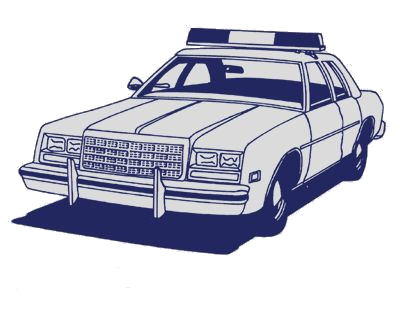
\includegraphics[width=0.5\textwidth]{./figures/logo.png}
\\[1cm]

\textsc{\LARGE TEAM RAMROD}\\[1.5cm]

\textsc{\Large Final Project Proposal}\\[0.5cm]

\HRule \\[0.4cm]
{\Huge \bfseries SNMP H4x0rZ}\\[0.4cm]
\HRule \\[1.5cm]

{\large
 \emph{Author:}\\
 Orion Miller\\
 Cameron Stearns\\
 Kellen Rogers\\
}

\vfill

{\large \today}

\end{center}
\end{titlepage}


\pagebreak

\setcounter{secnumdepth}{2}

\section{Scenario}
As Simple Network Management Protocol (SNMP) is commonly used to manage complex 
network resources, maintaining such a system is something that a small company 
may wish to outsource to a third party IT company.  This company would likely 
have a direct VPN to access the SNMP servers and clients running on the remote 
system, which we  will emulate as described below. The goal of this project 
is to highlight the insecurites of the SNMP protocol, its common configurations 
and its negative effects of being a part of management systems 
(e.g. a hardware management system.)

\section{Goal}
We plan to implement a proof of concept of a known Simple Network Management 
Protocol vulnerability over multiple atonomous systems. If there is enough time
we would like to find and implement a SNMP vulnerability of our own. We may attack
a different SNMPv3 vulnerability if our initially intended vulnerability does not work out.

\section{HMAC - Known SNMP Vulnerability}
SNMP, as of 2008, has a known bug with several implementations involving its use 
of a cryptographic-hash based authentication system (HMAC).  While this issue was 
patched in some implementations, non-updated systems and systems with certain 
software may still have this vulnerability.  Because the HMAC calculates an 
authentication code that may be as small as 1 byte, a process can quickly 
brute-force a code, and then produce traps to both read and modify any visible 
SNMP objects.
\\

\noindent The details of this weakness are outlined in the following articles
\begin{itemize}
\item \url{http://www.cisco.com/en/US/products/csa/cisco-sa-20080610-snmpv3.html}
\item \url{http://www.cert.org/advisories/CA-2002-03.html}
\end{itemize}


\section{Setup and Logistics}
In an overal structure for the completition of this project
we will need 3 main factors to be able to complete the project.
We need the Network setup, SNMP servers and clients and 
our tools to actively exploit the vulnerabilities in
SNMP.

\subsection{Network}
In this project, we hope to create a network involving 3 autonomous 
systems \emph{Figure 1}.  We will configure a middle AS as a transit  %% add figure link
network, and run a VPN between the other two autonomous systems.

\begin{figure}
  \centering
  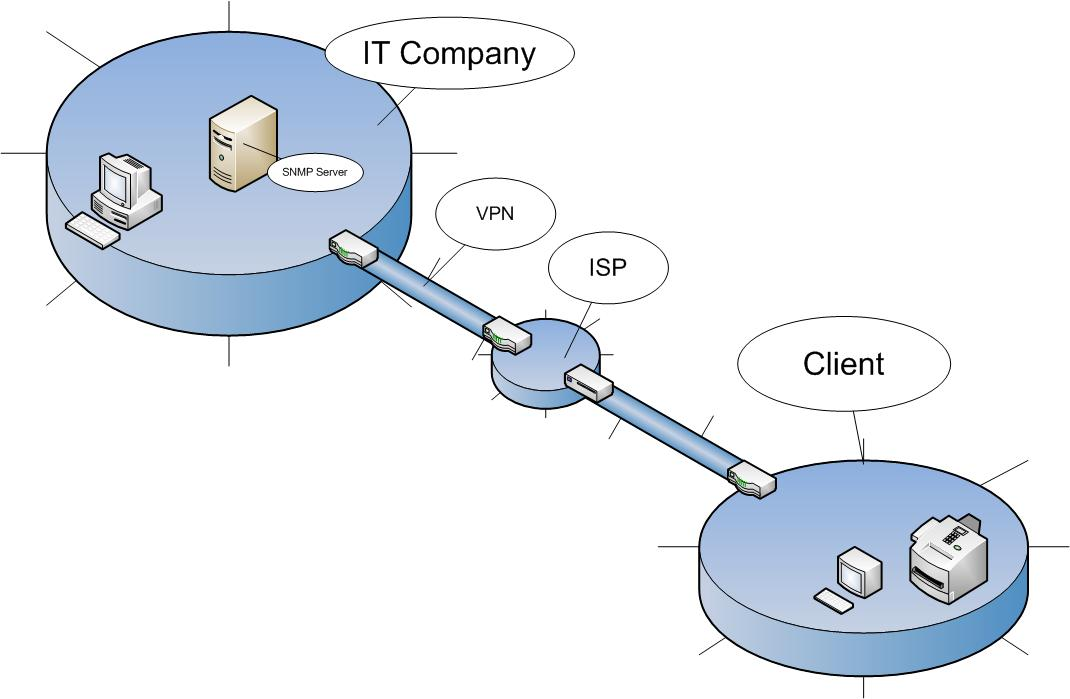
\includegraphics[width=0.95\textwidth, scale=1]{./figures/NetworkTopology.png}
  \caption{Proposed Network Topology}
\end{figure}

\subsection{SNMP}
Over this VPN, we will run the SNMP protocol, which has known 
implementation vulnerabilities as of SNMPv3. On the “IT” AS, we will 
run a server tasked with managing resources of the devices on our 
“Client” AS.  These resources will probably be things such as ink 
levels in a printer, or other easy to monitor resources.

\subsection{Attacks}
When we attempt to exploit SNMP vulnerabilities, we will perform our 
attacks from several topological locations in our network.  The most 
obvious first place to try would be in either the “Client” or “IT” AS; 
however, we would also like to show results for attempts made from 
the “ISP” AS and other external locations.

\section{Deliverables}

\begin{itemize}
\item Poster
  \subitem Abstract of final process
  \subitem Evaluation of attack successes, failures, and limitations
  \subitem Final network topology map (physical and logical)
  \subitem General description of our process and methods

\item Demo
  \subitem Fully running version of the network topology %link to figure example
  \subitem Fully running SNMPv3 servers and clients
  \subitem Visual presentation of the results of the attacks

\item Write-Up
  \subitem Goals
  \subitem What we completed
  \subitem Dummy corporate network in-depth explanation
  \subitem Step-by-Step explenation of SNMP Attacks
  \subitem How our tools were designed and how they work
  \subitem Network Configuration

\item Network Configuration
  \subitem Configuration files from each router
  \subitem Script of executed commands
  \subitem Final Logical Network Topology
  \subitem Final Real Network Topology

\item SNMP Attack Tools
  \subitem SNMP tools that take advantage of SNMPv3  vulnerabilities
  \subitem Provide the source code for said tools

\end{itemize}

\section{Deadlines}
\textit{All deadlines are tentative.}

\begin{center}
\begin{tabular}{l l}
  May 19 & SNMP Servers \& Clients Functional \\
  May 21 & SNMP Exploits Tools Functional \\
  May 23 & Network Setup \& Functional \\
  May 25 & Write-Up, Poster, \& Demo Completed \\
\end{tabular}
\end{center}




\end{document}
